\chapter{Additional Plots}\label{appendix:plots}
In this chapter we include some additional plots for the examples of
Section~\ref{sec:crqi:experiments}. We fix the following notation: $N$
denotes the order of the test matrix that was used in the respective
example, \ie the size of the matrix is $N \times N$. The (acute) angle
between the target eigenvector and the initial vector that was used in
the algorithm is denoted by $\alpha$ (the angle is always given in
degrees).

\begin{figure*}
  \centering
  \begin{subfigure}[t]{0.475\textwidth}
    \centering
    \includegraphics[width=\textwidth]{Figures/num_ex/ex1/mat_121/ex1_residuals_mat2_200_39_52-crop}
    \caption{{\small $N = 200\,, \alpha = 39.52^\circ$}}
  \end{subfigure}
  \hfill
  \begin{subfigure}[t]{0.475\textwidth}
    \centering
    \includegraphics[width=\textwidth]{Figures/num_ex/ex1/mat_121/ex1_residuals_mat2_1000_50_29-crop}
    \caption{{\small $N = 1000\,, \alpha = 50.29^\circ$}}
  \end{subfigure}
  \vskip\baselineskip
  \begin{subfigure}[t]{0.475\textwidth}
    \centering
    \includegraphics[width=\textwidth]{Figures/num_ex/ex1/mat_121/ex1_residuals_mat2_2000_49_11-crop}
    \caption{{\small $N = 2000\,, \alpha = 49.11^\circ$}}
  \end{subfigure}
  \hfill
  \begin{subfigure}[t]{0.475\textwidth}
    \centering
    \includegraphics[width=\textwidth]{Figures/num_ex/ex1/mat_121/ex1_residuals_mat2_4000_46_29-crop}
    \caption{{\small $N = 4000\,, \alpha = 46.29^\circ$}}
  \end{subfigure}
  \caption[Residuals for the {$[1,2,1]$} matrix]{Plot of the residual
    for different choices of imaginary shifts for the $[1,2,1]$
    matrix.}%
  \label{fig:imag_shift:mat2}
\end{figure*}

\begin{figure*}
  \centering
  \begin{subfigure}[t]{0.475\textwidth}
    \centering
    \includegraphics[width=\textwidth]{Figures/num_ex/ex1/mat_wilkinson/ex1_residuals_mat3_401_49_48-crop}
    \caption{{\small $N = 401\,, \alpha = 49.48^\circ$}}
  \end{subfigure}
  \hfill
  \begin{subfigure}[t]{0.475\textwidth}
    \centering
    \includegraphics[width=\textwidth]{Figures/num_ex/ex1/mat_wilkinson/ex1_residuals_mat3_1001_42_63-crop}
    \caption{{\small $N = 1001\,, \alpha = 42.63^\circ$}}
  \end{subfigure}
  \vskip\baselineskip
  \begin{subfigure}[t]{0.475\textwidth}
    \centering
    \includegraphics[width=\textwidth]{Figures/num_ex/ex1/mat_wilkinson/ex1_residuals_mat3_2001_45_29-crop}
    \caption{{\small $N = 2001\,, \alpha = 45.29^\circ$}}
  \end{subfigure}
  \hfill
  \begin{subfigure}[t]{0.475\textwidth}
    \centering
    \includegraphics[width=\textwidth]{Figures/num_ex/ex1/mat_wilkinson/ex1_residuals_mat3_3001_33_89-crop}
    \caption{{\small $N = 3001\,, \alpha = 33.89^\circ$}}
  \end{subfigure}
  \caption[Residuals for the Wilkinson matrix $\mat{W}^{+}$]{Plot of
    the residual for different choices of imaginary shifts for the
    Wilkinson matrix $\mat{W}^{+}$. The results using the squares
    residual norm as the imaginary shift are not included since in all
    cases the number of iterations was too high.}%
  \label{fig:imag_shift:mat3}
\end{figure*}

\begin{figure*}
  \centering
  \begin{subfigure}[t]{0.475\textwidth}
    \centering
    \includegraphics[width=\textwidth]{Figures/num_ex/ex1/mat_martin_wilkinson/ex1_residuals_mat4_1000_47_77-crop}
    \caption{{\small $N = 1000\,, \alpha = 47.77^\circ$}}
  \end{subfigure}
  \hfill
  \begin{subfigure}[t]{0.475\textwidth}
    \centering
    \includegraphics[width=\textwidth]{Figures/num_ex/ex1/mat_martin_wilkinson/ex1_residuals_mat4_2000_46_01-crop}
    \caption{{\small $N = 2000\,, \alpha = 46.01^\circ$}}
  \end{subfigure}
  \vskip\baselineskip
  \begin{subfigure}[t]{0.475\textwidth}
    \centering
    \includegraphics[width=\textwidth]{Figures/num_ex/ex1/mat_martin_wilkinson/ex1_residuals_mat4_4000_50_79-crop}
    \caption{{\small $N = 4000\,, \alpha = 50.79^\circ$}}
  \end{subfigure}
  \hfill
  \begin{subfigure}[t]{0.475\textwidth}
    \centering
    \includegraphics[width=\textwidth]{Figures/num_ex/ex1/mat_martin_wilkinson/ex1_residuals_mat4_5000_36_70-crop}
    {{\small $N = 5000\,, \alpha = 36.70^\circ$}}
  \end{subfigure}
  \caption[Residuals for the Martin-Wilkinson matrix $\mat{MW}$]{Plot
    of the residual for different choices of imaginary shifts for the
    Martin-Wilkinson matrix $\mat{MW}$.}%
  \label{fig:imag_shift:mat4}
\end{figure*}

\begin{figure*}
  \centering
  \begin{subfigure}[t]{0.475\textwidth}
    \centering
    \includegraphics[width=\textwidth]{Figures/num_ex/ex1/mat_laplace/ex1_residuals_mat5_625_39_12-crop.pdf}
    \caption{{\small $N = 625\,, \alpha = 39.12^\circ$}}
  \end{subfigure}
  \hfill
  \begin{subfigure}[t]{0.475\textwidth}
    \centering
    \includegraphics[width=\textwidth]{Figures/num_ex/ex1/mat_laplace/ex1_residuals_mat5_2500_49_05-crop}
    \caption{{\small $N = 2500\,, \alpha = 49.05^\circ$}}
  \end{subfigure}
  \vskip\baselineskip
  \begin{subfigure}[t]{0.475\textwidth}
    \centering
    \includegraphics[width=\textwidth]{Figures/num_ex/ex1/mat_laplace/ex1_residuals_mat5_5625_47_32-crop}
    \caption{{\small $N = 5625\,, \alpha = 47.32^\circ$}}
  \end{subfigure}
  \hfill
  \begin{subfigure}[t]{0.475\textwidth}
    \centering
    \includegraphics[width=\textwidth]{Figures/num_ex/ex1/mat_laplace/ex1_residuals_mat5_10000_43_89-crop}
    \caption{{\small $N = 10000\,, \alpha = 43.89^\circ$}}
  \end{subfigure}
  \caption[Residuals for the Laplace matrix]{Plot of the residual for
    different choices of imaginary shifts for the Laplace matrix.}%
  \label{fig:imag_shift:mat5}
\end{figure*}

%%%%%%%%%%%%%%%%%%%%%%%%%%%%%%%%%%%%%%%%%%%%%%%%%%%%%%%%%%%%%%%%%%
%%%%%%%%%%%%% EXAMPLE 2 %%%%%%%%%%%%%%%%%%%%%%%%%%%%%%%%%%%%%%%%%%
%%%%%%%%%%%%%%%%%%%%%%%%%%%%%%%%%%%%%%%%%%%%%%%%%%%%%%%%%%%%%%%%%%
\begin{figure*}
  \centering
  \begin{subfigure}[t]{0.475\textwidth}
    \centering
    \includegraphics[width=\textwidth]{Figures/num_ex/ex2/mat_121/ex2_rshift_mat2_1000_45_43.pdf}
    \caption{{\small $N = 1000\,, \alpha = 45.43^\circ$}}%
    \label{fig:real_shift:mat2:a}
  \end{subfigure}
  \hfill
  \begin{subfigure}[t]{0.475\textwidth}
    \centering
    \includegraphics[width=\textwidth]{Figures/num_ex/ex2/mat_121/ex2_rshift_mat2_4000_50_70}
    \caption{{\small $N = 4000\,, \alpha = 50.70^\circ$}}
  \end{subfigure}
  \vskip\baselineskip
  \begin{subfigure}[t]{0.475\textwidth}
    \centering
    \includegraphics[width=\textwidth]{Figures/num_ex/ex2/mat_121/ex2_rshift_mat2_4000_46_23}
    \caption{{\small $N = 4000\,, \alpha = 46.23^\circ$}}%
    \label{fig:real_shift:mat2:c}
  \end{subfigure}
  \hfill
  \begin{subfigure}[t]{0.475\textwidth}
    \centering
    \includegraphics[width=\textwidth]{Figures/num_ex/ex2/mat_121/ex2_rshift_mat2_1000_86_83}
    \caption{{\small $N = 1000\,, \alpha = 86.83^\circ$}}%
    \label{fig:real_shift:mat2:d}
  \end{subfigure}
  \caption[Effect of real shift for {$[1,2,1]$} matrix]{Plot of the
    computed eigenvalue against the initial real shift for the
    $[1,2,1]$ matrix.}%
  \label{fig:real_shift:mat2}
\end{figure*}

\begin{figure*}
  \centering
  \begin{subfigure}[t]{0.475\textwidth}
    \centering
    \includegraphics[width=\textwidth]{Figures/num_ex/ex2/mat_wilkinson/ex2_rshift_mat3_801_47_47}
    \caption{{\small $N = 801\,, \alpha = 47.47^\circ$}}
  \end{subfigure}
  \hfill
  \begin{subfigure}[t]{0.475\textwidth}
    \centering
    \includegraphics[width=\textwidth]{Figures/num_ex/ex2/mat_wilkinson/ex2_rshift_mat3_2001_36_78}
    \caption{{\small $N = 2001\,, \alpha = 36.78^\circ$}}
  \end{subfigure}
  \vskip\baselineskip
  \begin{subfigure}[t]{0.475\textwidth}
    \centering
    \includegraphics[width=\textwidth]{Figures/num_ex/ex2/mat_wilkinson/ex2_rshift_mat3_2001_45_82}
    \caption{{\small $N = 2001\,, \alpha = 45.82^\circ$}}
  \end{subfigure}
  \hfill
  \begin{subfigure}[t]{0.475\textwidth}
    \centering
    \includegraphics[width=\textwidth]{Figures/num_ex/ex2/mat_wilkinson/ex2_rshift_mat3_8001_43_69}
    \caption{{\small $N = 8001\,, \alpha = 43.69^\circ$}}
  \end{subfigure}
  \caption[Effect of real shift for the Wilkinson matrix
  $\mat{W}^{+}$]{Plot of the computed eigenvalue against the initial
    real shift for the Wilkinson matrix $\mat{W}^{+}$.}%
  \label{fig:real_shift:mat3}
\end{figure*}

\begin{figure*}
  \centering
  \begin{subfigure}[t]{0.475\textwidth}
    \centering
    \includegraphics[width=\textwidth]{Figures/num_ex/ex2/mat_martin_wilkinson/ex2_rshift_mat4_1000_24_58}
    \caption{{\small $N = 1000\,, \alpha = 24.58^\circ$}}
  \end{subfigure}
  \hfill
  \begin{subfigure}[t]{0.475\textwidth}
    \centering
    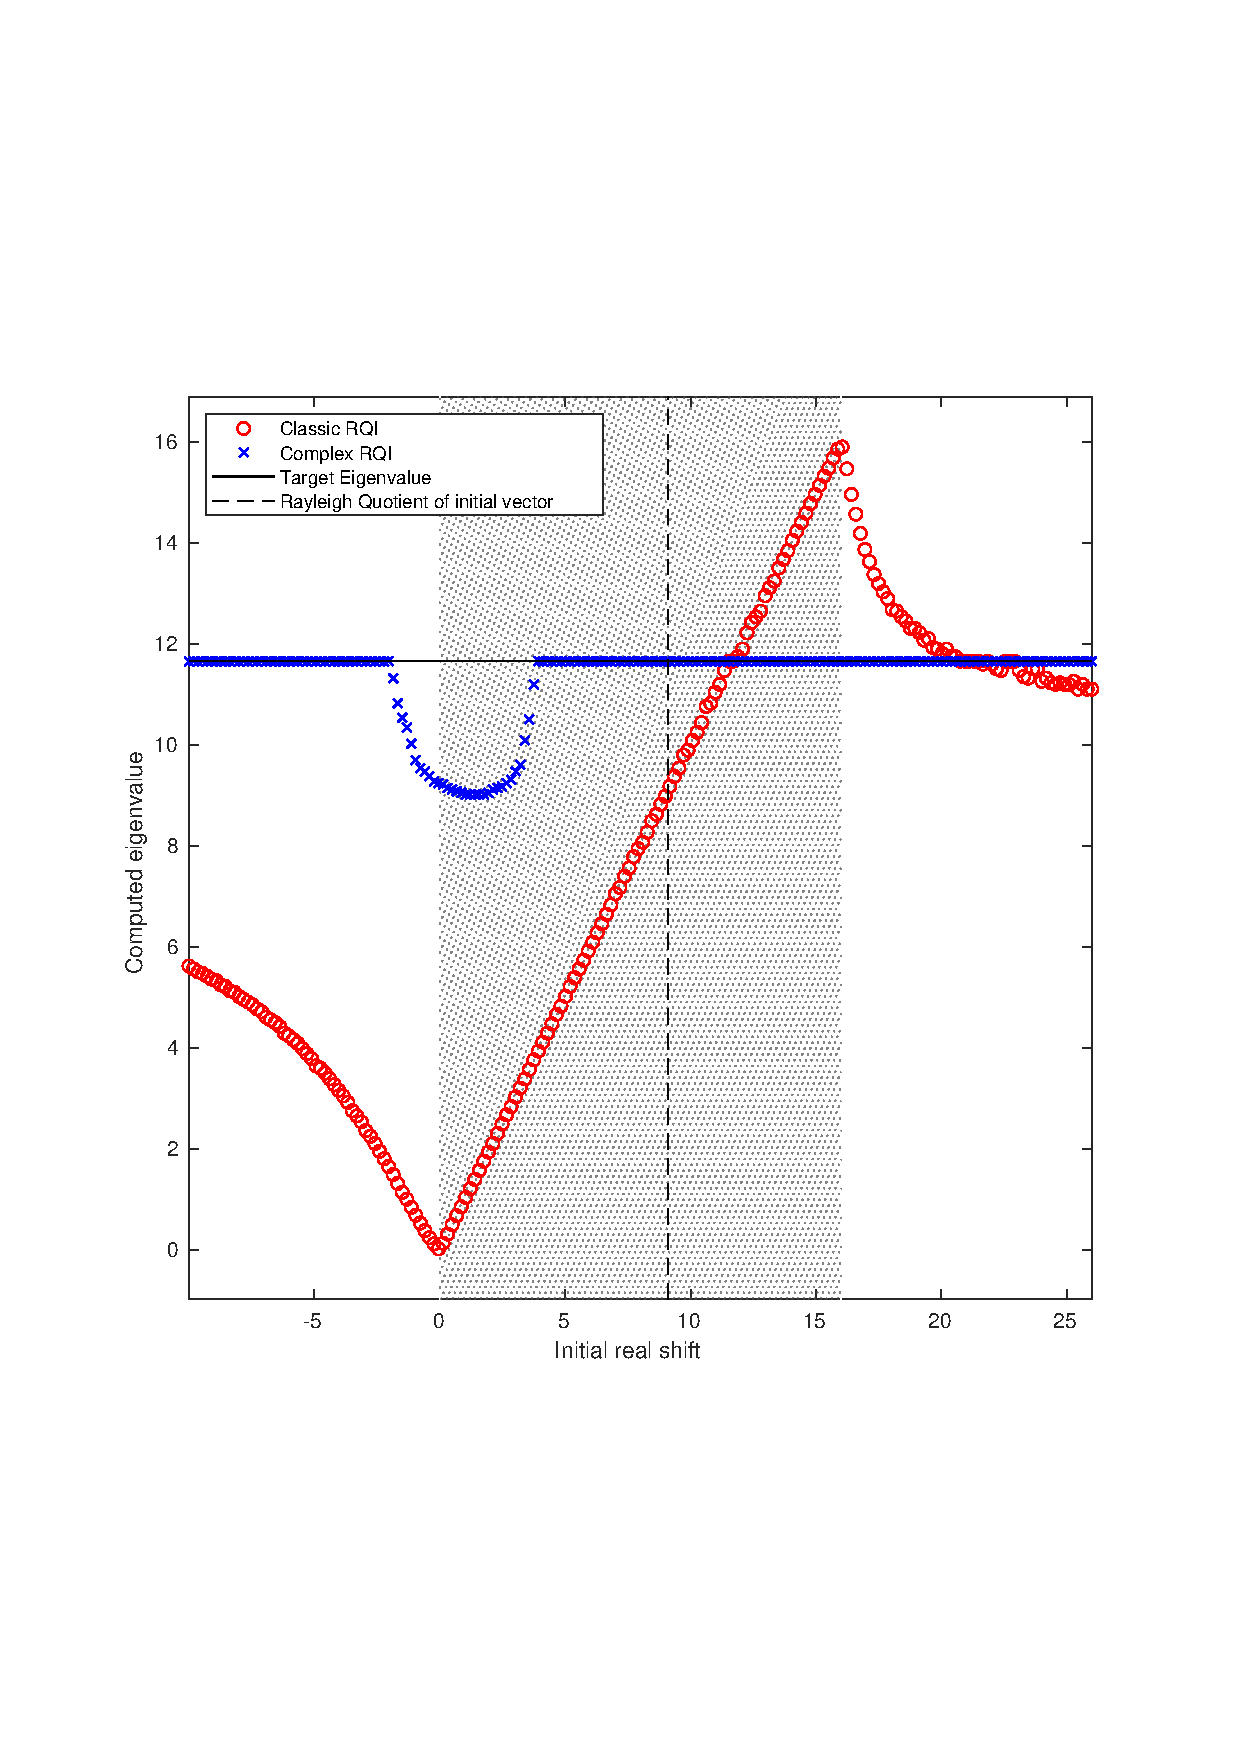
\includegraphics[width=\textwidth]{Figures/num_ex/ex2/mat_martin_wilkinson/ex2_rshift_mat4_1000_42_34}
    \caption{{\small $N = 1000\,, \alpha = 42.34^\circ$}}
  \end{subfigure}
  \vskip\baselineskip
  \begin{subfigure}[t]{0.475\textwidth}
    \centering
    \includegraphics[width=\textwidth]{Figures/num_ex/ex2/mat_martin_wilkinson/ex2_rshift_mat4_1000_50_13}
    \caption{{\small $N = 1000\,, \alpha = 50.13^\circ$}}
  \end{subfigure}
  \hfill
  \begin{subfigure}[t]{0.475\textwidth}
    \centering
    \includegraphics[width=\textwidth]{Figures/num_ex/ex2/mat_martin_wilkinson/ex2_rshift_mat4_8000_46_05}
    \caption{{\small $N = 8000\,, \alpha = 46.05^\circ$}}
  \end{subfigure}
  \caption[Effect of real shift for the Martin-Wilkinson matrix
  $\mat{MW}$]{Plot of the computed eigenvalue against the initial real
    shift for the Martin-Wilkinson matrix $\mat{MW}$.}%
  \label{fig:real_shift:mat4}
\end{figure*}

\begin{figure*}
  \centering
  \begin{subfigure}[t]{0.475\textwidth}
    \centering
    \includegraphics[width=\textwidth]{Figures/num_ex/ex2/mat_laplace/ex2_rshift_mat5_1600_48_92}
    \caption{{\small $N = 1600\,, \alpha = 48.92^\circ$}}
  \end{subfigure}
  \hfill
  \begin{subfigure}[t]{0.475\textwidth}
    \centering
    \includegraphics[width=\textwidth]{Figures/num_ex/ex2/mat_laplace/ex2_rshift_mat5_1600_44_96}
    \caption{{\small $N = 1600\,, \alpha = 44.96^\circ$}}
  \end{subfigure}
  \vskip\baselineskip
  \begin{subfigure}[t]{0.475\textwidth}
    \centering
    \includegraphics[width=\textwidth]{Figures/num_ex/ex2/mat_laplace/ex2_rshift_mat5_4900_38_78}
    \caption{{\small $N = 4900\,, \alpha = 38.78^\circ$}}
  \end{subfigure}
  \hfill
  \begin{subfigure}[t]{0.475\textwidth}
    \centering
    \includegraphics[width=\textwidth]{Figures/num_ex/ex2/mat_laplace/ex2_rshift_mat5_10000_37_46}
    \caption{{\small $N = 10000\,, \alpha = 37.46^\circ$}}
  \end{subfigure}
  \caption[Effect of real shift for the Laplace matrix]{Plot of the
    computed eigenvalue against the initial real shift for the Laplace
    matrix.}%
  \label{fig:real_shift:mat5}
\end{figure*}

%%%%%%%%%%%%%%%%%%%%%%%%%%%%%%%%%%%%%%%%%%%%%%%%%%%%%%%%%%%%%%%%%%
%%%%%%%%%%%%% EXAMPLE 3 %%%%%%%%%%%%%%%%%%%%%%%%%%%%%%%%%%%%%%%%%%
%%%%%%%%%%%%%%%%%%%%%%%%%%%%%%%%%%%%%%%%%%%%%%%%%%%%%%%%%%%%%%%%%%

\begin{figure*}
  \centering
  \begin{subfigure}[t]{0.475\textwidth}
    \centering
    \includegraphics[width=\textwidth]{Figures/num_ex/ex3/mat_121/ex3_angle_mat2_1000}
    \caption{{\small $N = 1000$}}
  \end{subfigure}
  \hfill
  \begin{subfigure}[t]{0.475\textwidth}
    \centering
    \includegraphics[width=\textwidth]{Figures/num_ex/ex3/mat_121/ex3_angle_mat2_2000}
    \caption{{\small $N = 2000$}}
  \end{subfigure}
  \vskip\baselineskip
  \begin{subfigure}[t]{0.475\textwidth}
    \centering
    \includegraphics[width=\textwidth]{Figures/num_ex/ex3/mat_121/ex3_angle_mat2_4000}
    \caption{{\small $N = 4000$}}
  \end{subfigure}
  \hfill
  \begin{subfigure}[t]{0.475\textwidth}
    \centering
    \includegraphics[width=\textwidth]{Figures/num_ex/ex3/mat_121/ex3_angle_mat2_8000}
    \caption{{\small $N = 8000$}}
  \end{subfigure}
  \caption[Effect of the angle between the initial vector and the
  target for the matrix {$[1,2,1]$}]{Plot of the computed eigenvalue
    against the angle between the initial vector and the target
    eigenvector for the matrix $[1,2,1]$.}%
  \label{fig:angle:mat2}
\end{figure*}

\begin{figure*}
  \centering
  \begin{subfigure}[t]{0.475\textwidth}
    \centering
    \includegraphics[width=\textwidth]{Figures/num_ex/ex3/mat_wilkinson/ex3_angle_mat3_2001}
    \caption{{\small $N = 2001$}}
  \end{subfigure}
  \hfill
  \begin{subfigure}[t]{0.475\textwidth}
    \centering
    \includegraphics[width=\textwidth]{Figures/num_ex/ex3/mat_wilkinson/ex3_angle_mat3_4001}
    \caption{{\small $N = 4001$}}
  \end{subfigure}
  \vskip\baselineskip
  \begin{subfigure}[t]{0.475\textwidth}
    \centering
    \includegraphics[width=\textwidth]{Figures/num_ex/ex3/mat_wilkinson/ex3_angle_mat3_8001}
    \caption{{\small $N = 8001$}}
  \end{subfigure}
  \hfill
  \begin{subfigure}[t]{0.475\textwidth}
    \centering
    \includegraphics[width=\textwidth]{Figures/num_ex/ex3/mat_wilkinson/ex3_angle_mat3_10001}
    \caption{{\small $N = 10001$}}
  \end{subfigure}
  \caption[Effect of the angle between the initial vector and the
  target for the Wilkinson matrix {$\mat{W}^{+}$}]{Plot of the
    computed eigenvalue against the angle between the initial vector
    and the target eigenvector for the Wilkinson matrix
    $\mat{W}^{+}$.}%
  \label{fig:angle:mat3}
\end{figure*}

\begin{figure*}
  \centering
  \begin{subfigure}[t]{0.475\textwidth}
    \centering
    \includegraphics[width=\textwidth]{Figures/num_ex/ex3/mat_martin_wilkinson/ex3_angle_mat4_2000}
    \caption{{\small $N = 2000$}}
  \end{subfigure}
  \hfill
  \begin{subfigure}[t]{0.475\textwidth}
    \centering
    \includegraphics[width=\textwidth]{Figures/num_ex/ex3/mat_martin_wilkinson/ex3_angle_mat4_4000}
    \caption{{\small $N = 4000$}}
  \end{subfigure}
  \vskip\baselineskip
  \begin{subfigure}[t]{0.475\textwidth}
    \centering
    \includegraphics[width=\textwidth]{Figures/num_ex/ex3/mat_martin_wilkinson/ex3_angle_mat4_8000}
    \caption{{\small $N = 8000$}}
  \end{subfigure}
  \hfill
  \begin{subfigure}[t]{0.475\textwidth}
    \centering
    \includegraphics[width=\textwidth]{Figures/num_ex/ex3/mat_martin_wilkinson/ex3_angle_mat4_10000}
    \caption{{\small $N = 10000$}}
  \end{subfigure}
  \caption[Effect of the angle between the initial vector and the
  target for the Martin-Wilkinson matrix {$\mat{MW}$}]{Plot of the
    computed eigenvalue against the angle between the initial vector
    and the target eigenvector for the Martin-Wilkinson matrix
    {$\mat{MW}$}.}%
  \label{fig:angle:mat4}
\end{figure*}

%%%%%%%%%%%%%%%%%%%%%%%%%%%%%%%%%%%%%%%%%%%%%%%%%%%%%%%%%%%%%%%%%%
%%%%%%%%%%%%% EXAMPLE 4 %%%%%%%%%%%%%%%%%%%%%%%%%%%%%%%%%%%%%%%%%%
%%%%%%%%%%%%%%%%%%%%%%%%%%%%%%%%%%%%%%%%%%%%%%%%%%%%%%%%%%%%%%%%%%
\begin{figure*}
  \centering
  \begin{subfigure}[t]{0.475\textwidth}
    \centering
    \includegraphics[width=\textwidth]{Figures/num_ex/ex4/mat_121/ex4_angle_mat2_2000}
    \caption{{\small $N = 2000$}}%
    \label{fig:ex4:mat2:a}
  \end{subfigure}
  \hfill
  \begin{subfigure}[t]{0.475\textwidth}
    \centering
    \includegraphics[width=\textwidth]{Figures/num_ex/ex4/mat_121/ex4_angle_mat2_4000}
    \caption{{\small $N = 4000$}}
  \end{subfigure}
  \vskip\baselineskip
  \begin{subfigure}[t]{0.475\textwidth}
    \centering
    \includegraphics[width=\textwidth]{Figures/num_ex/ex4/mat_121/ex4_angle_mat2_8000}
    \caption{{\small $N = 8000$}}%
  \end{subfigure}
  \hfill
  \begin{subfigure}[t]{0.475\textwidth}
    \centering
    \includegraphics[width=\textwidth]{Figures/num_ex/ex4/mat_121/ex4_angle_mat2_10000_e_3_999}
    \caption{{\small $N = 10000$. Target eigenvalue was close to the
        upper end of the spectrum ($\lambda \approx 3.999$).}}%
    \label{fig:ex4:mat2:fail}
  \end{subfigure}
  \caption[Number of iterations for different angles for the
  {$[1,2,1]$} matrix]{Plot of the number of iterations of classic RQI
    and complex RQI for the {$[1,2,1]$} matrix.}%
  \label{fig:ex4:mat2}
\end{figure*}

\begin{figure*}
  \centering
  \begin{subfigure}[t]{0.475\textwidth}
    \centering
    \includegraphics[width=\textwidth]{Figures/num_ex/ex4/mat_wilkinson/ex4_angle_mat3_2001}
    \caption{{\small $N = 2001$}}
  \end{subfigure}
  \hfill
  \begin{subfigure}[t]{0.475\textwidth}
    \centering
    \includegraphics[width=\textwidth]{Figures/num_ex/ex4/mat_wilkinson/ex4_angle_mat3_4001}
    \caption{{\small $N = 4001$}}
  \end{subfigure}
  \vskip\baselineskip
  \begin{subfigure}[t]{0.475\textwidth}
    \centering
    \includegraphics[width=\textwidth]{Figures/num_ex/ex4/mat_wilkinson/ex4_angle_mat3_8001}
    \caption{{\small $N = 8001$}}
  \end{subfigure}
  \hfill
  \begin{subfigure}[t]{0.475\textwidth}
    \centering
    \includegraphics[width=\textwidth]{Figures/num_ex/ex4/mat_wilkinson/ex4_angle_mat3_10001}
    \caption{{\small $N = 10001$}}%
    \label{fig:ex4:mat3:d}
  \end{subfigure}
  \caption[Number of iterations for different angles for the Wilkinson
  matrix $\mat{W}^{+}$]{Plot of the number of iterations of classic
    RQI and complex RQI for the Wilkinson matrix $\mat{W}^{+}$.}%
  \label{fig:ex4:mat3}
\end{figure*}

\begin{figure*}
  \centering
  \begin{subfigure}[t]{0.475\textwidth}
    \centering
    \includegraphics[width=\textwidth]{Figures/num_ex/ex4/mat_martin_wilkinson/ex4_angle_mat4_2000}
    \caption{{\small $N = 2000$}}
  \end{subfigure}
  \hfill
  \begin{subfigure}[t]{0.475\textwidth}
    \centering
    \includegraphics[width=\textwidth]{Figures/num_ex/ex4/mat_martin_wilkinson/ex4_angle_mat4_4000_fail}
    \caption{{\small $N = 4000$. Target eigenvalue was close to the
        lower end of the spectrum ($\lambda \approx 0.000717$).}}%
    \label{fig:ex4:mat4:fail}
  \end{subfigure}
  \vskip\baselineskip
  \begin{subfigure}[t]{0.475\textwidth}
    \centering
    \includegraphics[width=\textwidth]{Figures/num_ex/ex4/mat_martin_wilkinson/ex4_angle_mat4_8000}
    \caption{{\small $N = 8000$}}
  \end{subfigure}
  \hfill
  \begin{subfigure}[t]{0.475\textwidth}
    \centering
    \includegraphics[width=\textwidth]{Figures/num_ex/ex4/mat_martin_wilkinson/ex4_angle_mat4_12000}
    \caption{{\small $N = 12000$}}%
    \label{fig:ex4:mat4:d}
  \end{subfigure}
  \caption[Number of iterations for different angles for the
  Martin-Wilkinson matrix $\mat{MW}$]{Plot of the number of iterations
    of classic RQI and complex RQI for the Martin-Wilkinson matrix
    $\mat{MW}$.}%
  \label{fig:ex4:mat4}
\end{figure*}

\begin{figure*}
  \centering
  \begin{subfigure}[t]{0.475\textwidth}
    \centering
    \includegraphics[width=\textwidth]{Figures/num_ex/ex4/mat_laplace/ex4_angle_mat5_2500}
    \caption{{\small $N = 2500$}}
  \end{subfigure}
  \hfill
  \begin{subfigure}[t]{0.475\textwidth}
    \centering
    \includegraphics[width=\textwidth]{Figures/num_ex/ex4/mat_laplace/ex4_angle_mat5_5625}
    \caption{{\small $N = 5625$}}
  \end{subfigure}
  \vskip\baselineskip
  \begin{subfigure}[t]{0.475\textwidth}
    \centering
    \includegraphics[width=\textwidth]{Figures/num_ex/ex4/mat_laplace/ex4_angle_mat5_6400}
    \caption{{\small $N = 6400$}}
  \end{subfigure}
  \hfill
  \begin{subfigure}[t]{0.475\textwidth}
    \centering
    \includegraphics[width=\textwidth]{Figures/num_ex/ex4/mat_laplace/ex4_angle_mat5_10000}
    \caption{{\small $N = 10000$}}
  \end{subfigure}
  \caption[Number of iterations for different angles for the Laplace
  matrix]{Plot of the number of iterations of classic RQI and complex
    RQI for the Laplace matrix.}%
  \label{fig:ex4:mat5}
\end{figure*}

%%% Local Variables:
%%% mode: latex
%%% TeX-master: "../../main"
%%% End:

